\documentclass[oneside,13pt,a4paper]{report}

% Chargement d'extensions
\usepackage[utf8]{inputenc}
\usepackage[french]{babel}
% csquotes va utiliser la langue définie dans babel
\usepackage[babel=true]{csquotes}
\usepackage[T1]{fontenc}
\usepackage{graphicx}
\usepackage[top=3cm, bottom=3cm, left=3cm, right=3cm]{geometry}
\usepackage{amsmath}
\usepackage{amssymb}


% Liens et autres
\usepackage{hyperref}
\hypersetup{
    colorlinks=true,
    linkcolor=black,
	urlcolor=blue,
	pdftitle={Rendu},
	bookmarks=true,
}

% Bout de code
\usepackage{listings}
\usepackage{color}

\definecolor{mygreen}{rgb}{0,0.6,0}
\definecolor{mygray}{rgb}{0.5,0.5,0.5}
\definecolor{mymauve}{rgb}{0.58,0,0.82}

\lstset{
  backgroundcolor=\color{white},   % choose the background color; you must add \usepackage{color} or \usepackage{xcolor}; should come as last argument
  basicstyle=\footnotesize,        % the size of the fonts that are used for the code
  breakatwhitespace=false,         % sets if automatic breaks should only happen at whitespace
  breaklines=true,                 % sets automatic line breaking
  captionpos=b,                    % sets the caption-position to bottom
  commentstyle=\color{mygreen},    % comment style
  deletekeywords={...},            % if you want to delete keywords from the given language
  escapeinside={\%*}{*)},          % if you want to add LaTeX within your code
  extendedchars=true,              % lets you use non-ASCII characters; for 8-bits encodings only, does not work with UTF-8
  firstnumber=0,                   % start line enumeration with line 1000
  frame=single,	                   % adds a frame around the code
  keepspaces=true,                 % keeps spaces in text, useful for keeping indentation of code (possibly needs columns=flexible)
  keywordstyle=\color{blue},       % keyword style
  %language=C++,                    % the language of the code
  morekeywords={*,...},            % if you want to add more keywords to the set
  numbers=left,                    % where to put the line-numbers; possible values are (none, left, right)
  numbersep=5pt,                   % how far the line-numbers are from the code
  numberstyle=\tiny\color{mygray}, % the style that is used for the line-numbers
  rulecolor=\color{black},         % if not set, the frame-color may be changed on line-breaks within not-black text (e.g. comments (green here))
  showspaces=false,                % show spaces everywhere adding particular underscores; it overrides 'showstringspaces'
  showstringspaces=false,          % underline spaces within strings only
  showtabs=false,                  % show tabs within strings adding particular underscores
  stepnumber=1,                    % the step between two line-numbers. If it's 1, each line will be numbered
  stringstyle=\color{mymauve},     % string literal style
  tabsize=2,	                   % sets default tabsize to 2 spaces
  literate=
  {á}{{\'a}}1 {é}{{\'e}}1 {í}{{\'i}}1 {ó}{{\'o}}1 {ú}{{\'u}}1
  {Á}{{\'A}}1 {É}{{\'E}}1 {Í}{{\'I}}1 {Ó}{{\'O}}1 {Ú}{{\'U}}1
  {à}{{\`a}}1 {è}{{\`e}}1 {ì}{{\`i}}1 {ò}{{\`o}}1 {ù}{{\`u}}1
  {À}{{\`A}}1 {È}{{\'E}}1 {Ì}{{\`I}}1 {Ò}{{\`O}}1 {Ù}{{\`U}}1
  {ä}{{\"a}}1 {ë}{{\"e}}1 {ï}{{\"i}}1 {ö}{{\"o}}1 {ü}{{\"u}}1
  {Ä}{{\"A}}1 {Ë}{{\"E}}1 {Ï}{{\"I}}1 {Ö}{{\"O}}1 {Ü}{{\"U}}1
  {â}{{\^a}}1 {ê}{{\^e}}1 {î}{{\^i}}1 {ô}{{\^o}}1 {û}{{\^u}}1
  {Â}{{\^A}}1 {Ê}{{\^E}}1 {Î}{{\^I}}1 {Ô}{{\^O}}1 {Û}{{\^U}}1
  {Ã}{{\~A}}1 {ã}{{\~a}}1 {Õ}{{\~O}}1 {õ}{{\~o}}1
  {œ}{{\oe}}1 {Œ}{{\OE}}1 {æ}{{\ae}}1 {Æ}{{\AE}}1 {ß}{{\ss}}1
  {ű}{{\H{u}}}1 {Ű}{{\H{U}}}1 {ő}{{\H{o}}}1 {Ő}{{\H{O}}}1
  {ç}{{\c c}}1 {Ç}{{\c C}}1 {ø}{{\o}}1 {å}{{\r a}}1 {Å}{{\r A}}1
  {€}{{\euro}}1 {£}{{\pounds}}1 {«}{{\guillemotleft}}1
  {»}{{\guillemotright}}1 {ñ}{{\~n}}1 {Ñ}{{\~N}}1 {¿}{{?`}}1
}

% Commande pour notation 'NB :' (nota bene)
\newcommand\nb[1][0.3]{N\kern-#1emB : }

% Espacement entre les paragraphes
\parskip=5pt

% pour afficher Schéma au lieu de figure dans les legende des images
\addto\captionsfrench{\def\figurename{Schéma}}

% Informations le titre, le(s) auteur(s), la date
\title{TITRE}
\author{
    Belkassim BOUZIDI \and
    Mélissa DADI  \and
    Chakib ELHOUITI \and
    Massili KEZZOUL \and
    Ramzi ZEROUAL
}
\date{\today}


\begin{document}
%\maketitle
\begin{titlepage}
	\centering
	{\scshape\LARGE Universite de Montpellier\par}
	{\scshape\Large Rapport de projet\par}
	\vspace{1.5cm}
	{\huge\bfseries TITRE\par}
	\vspace{2cm}
	{\Large\itshape
		Belkassim BOUZIDI \\
    	Mélissa DADI \\
		Chakib ELHOUITI \\
		Massili KEZZOUL \\
		Ramzi ZEROUAL \\
		\par}

	\vspace{1.5cm}

	{\Large\itshape
		Encadrant :\par
		M. Pascal \textsc{Poncelet}
		\par}

	\vspace{2cm}

	\begin{figure}[h]
		\begin{minipage}[c]{.46\linewidth}
			\centering
			
\includegraphics[width=1\textwidth]{img/univ-montpellier.png}
		\end{minipage}
		\hfill%
		\begin{minipage}[c]{.46\linewidth}
			\centering
			
\includegraphics[width=1\textwidth]{img/fds.png}
		\end{minipage}
	\end{figure}

	\par\vspace{1cm}

	\vfill

	% Bottom of the page
	{\large \today\par}
\end{titlepage}

% ------------------------------------- %
% Introduction
% ------------------------------------- %

\parskip=5pt
\chapter*{Remerciements}
\vspace{\stretch{1}}
\begin{center}

	Tout d'abord nous souhaitons adresser nos remerciements au corps professoral et administratif de la faculté des sciences de Montpellier qui déploient des efforts pour assurer à leurs étudiants une formation actualisée.

	En second lieu, nous tenons à remercier notre encadrant M. Pascal \textsc{Poncelet} pour ses précieux conseils et son aide durant toute la période de travail.

	Nos vifs remerciements vont également aux membres du jury pour l’intérêt qu’ils ont porté à notre projet en acceptant d’examiner notre travail.

	Nous remercions M. Yahia Zeroual pour sa relecture attentive de ce rapport.

\end{center}
\vspace{\stretch{1}}

\parskip=0pt
\tableofcontents

% Espacement entre les paragraphes
\parskip=5pt


% ------------------------------------- %
% Introduction au sujet
% ------------------------------------- %

\chapter{Introduction au sujet}

\section{Les réseaux de neurones pronfonds}

En termes simples, le Deep Learning est le domaine où les machines apprennent par elles-mêmes en imitant le cerveau humain. Imiter dans le sens où les machines peuvent effectuer des tâches nécessitant une intelligence humaine. Maintenant, comprenons comment ?


\begin{figure}[!h]
	\begin{center}
		 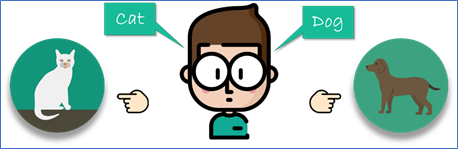
\includegraphics[width=0.7\textwidth]{img/intro1.png}
		 \caption{}
	\end{center}
\end{figure}

Le cerveau humain peut facilement différencier un chat et un chien.

\begin{figure}[!h]
	\begin{center}
		 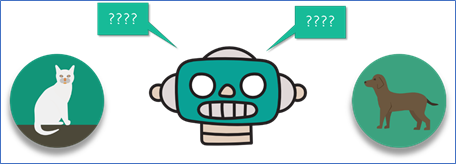
\includegraphics[width=0.7\textwidth]{img/intro2.png}
		 \caption{}
	\end{center}
\end{figure}

Mais comment faire différencier une machine entre un chat et un chien ?
\begin{figure}[!h]
	\begin{center}
		 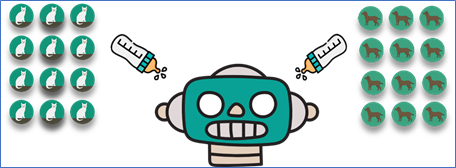
\includegraphics[width=0.7\textwidth]{img/intro3.png}
		 \caption{}
	\end{center}
\end{figure}

La majorité des méthodes d'apprentissage profond utilisent des architectures de réseau neuronal et c'est pourquoi les modèles d'apprentissage profond sont également connus sous le nom de réseaux neuronaux profonds.
Un processus d'apprentissage en profondeur se compose de deux phases clé : l’entraînement et l'inférence.

La phase d' entrainement peut être considérée comme un processus d'étiquetage d'énormes quantités de données et d'identification de leurs caractéristiques correspondantes. Ici, le système compare ces caractéristiques et les mémorise pour arriver à des conclusions correctes lorsqu'il rencontre des données similaires la prochaine fois.

Au cours de la phase d'inférence, le modèle tire des conclusions et étiquette les données non exposées à l'aide des connaissances acquises précédemment.

\paragraph{Des exemples : }

Un grand nombre d'industries utilisent le deep learning pour tirer parti de ses avantages. Jetons un coup d'œil à quelques-uns d'entre eux.

\begin{description}
	\item[Électronique] l'apprentissage en profondeur est utilisé dans la traduction automatique de la parole. Vous pouvez penser aux appareils d'assistance à domicile qui répondent à votre voix et comprennent vos préférences.
	\item[Conduite automatisée] grâce à l'apprentissage en profondeur, les chercheurs automobiles sont désormais en mesure de détecter automatiquement des objets tels que les feux de signalisation, les panneaux d'arrêt, etc. Ils l'utilisent également pour détecter les piétons, ce qui contribue à réduire les accidents.
	\item[Recherche médicale] l'apprentissage en profondeur est utilisé par les chercheurs en cancérologie pour détecter automatiquement les cellules cancéreuses.
\end{description}

Si les réseaux de neurones profonds obtiennent souvent des bons résultats, ils ont cependant un point faible : leur fonctionnement apparaît comme bien plus opaque. Un phénomène appelé « boîte noire » (« black box » en anglais), dans le sens où l'on peut juger des données qui entrent dans la boîte et des résultats qui en sortent, mais sans savoir ce qui se passe à l'intérieur.

\section{Jeu de données}

Nous avons choisi d'utiliser la base de données MNIST\footnote{Modified ou Mixed National Institute of Standards and Technology} comme jeu de données. L'ensemble de données MNIST est l'un des ensembles de données les plus couramment utilisés pour la classification d'images et accessible à partir de nombreuses sources différentes. Tensorflow nous permet d'importer et de télécharger le jeu de données directement depuis leur API.

La base de données MNIST, une extension de la base de données NIST, est une collection de données de faible complexité de chiffres manuscrits utilisés pour entraîner divers algorithmes d'apprentissage automatique supervisées. MNIST est considéré comme le \textit{Hello world} de l'apprentissage automatique.

MNIST est un ensemble de données étiqueté qui associe des images de chiffres écrits à la main avec la valeur du chiffre respectif. Elle contient 70 000 images en noir et blanc de 28 x 28 pixels représentant des chiffres de zéro à neuf. Chaque pixel de l'image est un entier de valeur comprise entre 0 et 255 représentant le niveau de gris.

\begin{figure}[!h]
	\begin{center}
		 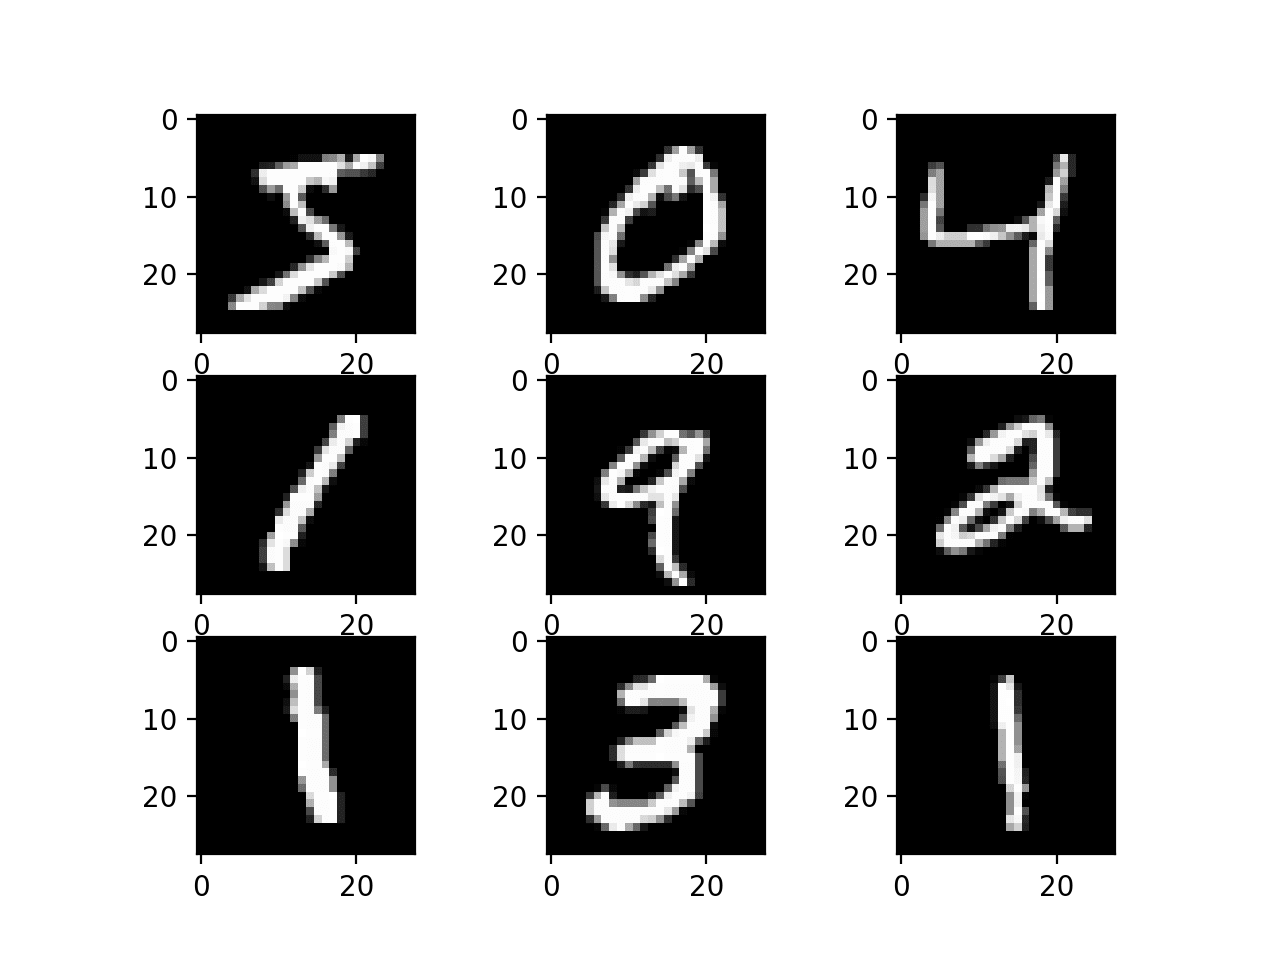
\includegraphics[width=0.7\textwidth]{img/mnist.png}
		 \caption{Exemple de quelques éléments de la base de données MNIST}
	\end{center}
\end{figure}

\section{Problèmatique}

L'objectif du projet est d'essayer de mieux comprendre le fonctionnement interne d'un réseau de neurones. Il s'agit de repérer, selon les données d'entrée, des signatures d'activation de neurones. Une signature correspond au pattern (ou chemin) emprunté par un objet au sein du réseau avant d'arriver à une conclusion. Concrètement, on veut analyser les différentes signatures obtenues par différents types de données et de modèles.

Par exemple, si on entraîne un modèle à reconnaître des images de \textit{chiens} et de \textit{chats}, on voudrait répondre aux questions suivantes :

\begin{itemize}
	\item À partir de quelle couche le modèle change de comportement pour reconnaître une image ?
	\item Les signatures des images de \textit{chats}, sont-elles différentes de ceux des \textit{chiens} ?
	\item Si on passe une image de \textit{voiture} au modèle, à quoi va ressembler sa signature ?
\end{itemize}

\section{Solution proposée}

Dans un premier temps, on doit se familiariser avec la base de données MNIST et développer plusieurs outils afin de les manipuler. Ensuite, nous passerons à la construction des modèles d'apprentissage pour pouvoir analyser leurs comportements internes en récupérant les soties de chaque couche cachée. À partir de ces sorties, l'objectif sera d'extraire les signatures grâce à des algorithmes de \textit{clustering}\footnote{Méthode en analyse des données. Elle vise à diviser un ensemble de données en différents paquets (\textit{clusters}) tel que chaque sous-ensemble partagent des caractéristiques communes.}. Enfin, nous réaliserons une interface de visualisation afin d'analyser les résultats et de répondre aux questions posées ci-dessus.

% ------------------------------------- %
% Organisation
% ------------------------------------- %

\chapter{Organisation du projet}
\section{Méthodes d’organisation}

Afin de mener à bien le développement du projet, nous avons décidé de travailler un maximum de temps ensemble et de manière très régulière. Nous nous sommes réunis deux à trois fois par semaine, en vue de faire le point sur l'avancement du projet et de définir les objectifs restants à atteindre.

Ainsi, selon l'état de progression du projet, nous réalisâmes les tâches en retard durant le week-end pour ne pas cumuler de retard et respecter l'intégralité du cahier des charges.

Toutes les deux semaines, nous nous sommes réunis avec notre encadrant, M. Pascal \textsc{Poncelet}. Lors de ces réunions de mises au point relatif au projet, de précieux conseils nous furent prodigués.

\section{Découpage du projet}

Nous avons découpé la réalisation du projet en trois grandes phases :

\subsection{Phase d'analyse des données}

Durant cette étape, nous nous sommes concentrés sur l'analyse des données que nous allions utiliser. Notamment l'étude de leur structure ainsi que la définition des différents outils utiles pour leur manipulation. Nous avons également choisi les outils de travail collaboratifs et les principales technologies utilisées.

\subsection{Phase de développement}

Durant cette phase, nous avons commencé à implémenter plusieurs modèles d'apprentissage automatique, les outils d'extraction des informations internes à ce dernier ainsi que les interfaces de visualisation des résultats.

\subsection{Phase d'analyse et présentation des résultats}

Cette étape a consisté en l'analyse des résultats obtenues durant la phase précédente. Nous nous sommes aussi penché sur la réalisation d'une interface web afin d'effectuer des expérimentations et de pouvoir, le plus intuitivement possible, visualiser les résultats.

\section{Outils de collaboration}

Afin de s'organiser, nous avons décidé d'utiliser le logiciel \textit{Git} à travers le serveur \textit{Github}. En effet le logiciel libre a facilité grandement la collaboration entre nous. Vous trouverez d'ailleurs l'intégralité du code source sur ce \href{https://github.com/massykezzoul/mtq-neural-networks}{depôt Github}.

En ce qui concerne la rédaction de ce rapport, nous avons utilisé \LaTeX, système de composition de documents créé par Leslie Lamport, pour faciliter la rédaction à plusieurs.

\begin{figure}[h]
	\begin{minipage}[c]{.46\linewidth}
		\centering
		
\includegraphics[width=1\textwidth]{img/github.png}
		\caption{Logo du GitLab}
	\end{minipage}
	\hfill%
	\begin{minipage}[c]{.46\linewidth}
		\centering
		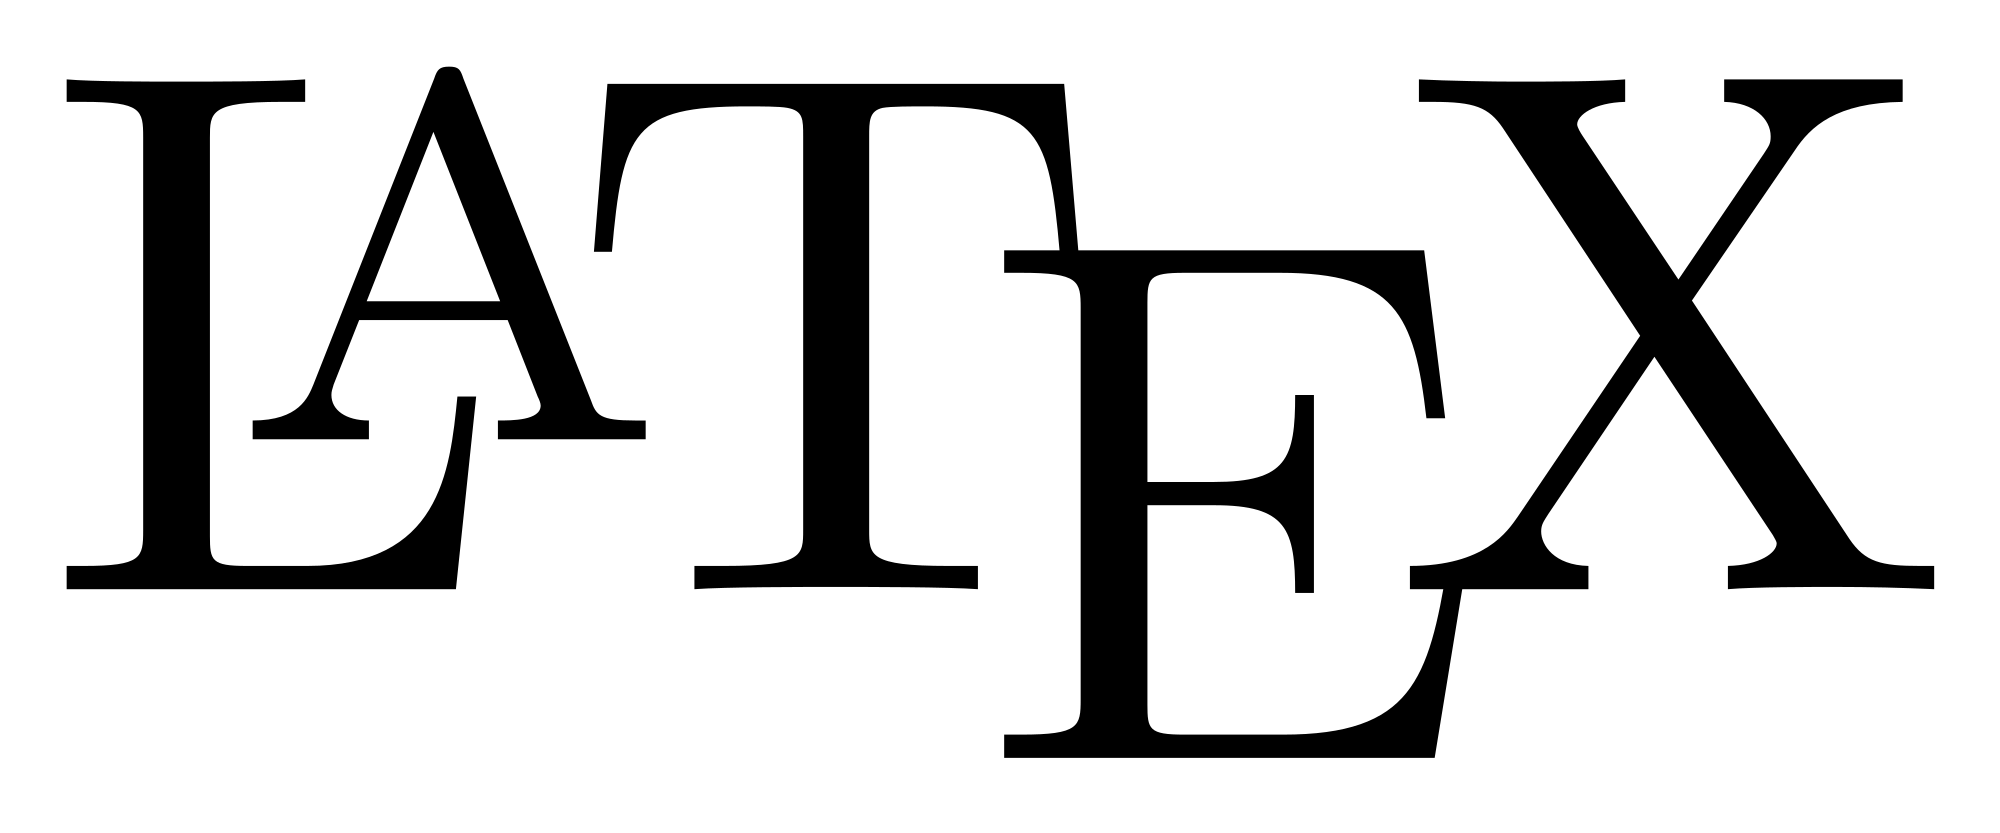
\includegraphics[width=1\textwidth]{img/latex.png}
		\caption{Logo de Latex}
	\end{minipage}
\end{figure}

% ------------------------------------- %
% Analyse des données
% ------------------------------------- %


\chapter{Analyse des données}

En récupérant les données brutes de \textit{MNIST}, qui sont des images de 28 x 28 pixels stockées sous la forme d'une matrice de 2 dimensions, avec une valeur entre 0 et 255 pour chaque case. Il est clair \textbf{qu'on ne peut pas} passer ces données à un réseau de neurones, vu que le réseau de neurones prends en input layer un tableau à une seule dimension.
Pour pouvoir traiter, entraîner et visualiser ces données, on a mis en place une série de prétraitements.

\section{Prétraitements} 

\subsection{Découpage des données}

Cette partie se résume par la fonction \textit{cut\_data}, qui nous permet de découper les données et garder un nombre précis d'images pour un ensemble de chiffres définis. Par exemple, on peut garder 100 images représentants des 0 et des 1 (100 pour chaque chiffre). On a réalisé cette fonction pour faciliter la phase de développement et de pouvoir mieux visualiser les résultats sur un petit ensemble de données.
\subsection{Scaling, Flattening}

La phase de prétraitements est la plus importante dans le processus de création d’un réseau neuronal. Pour cela, on a mis en place
la fonction \textit{normalize\_dataset} qui fait, en premier du Scaling (standardisation ou normalisation et c'est ce qu'on a utilisé dans notre cas), qui consiste à mettre les valeurs des images entre 0 et 1 au lieu de 0 et 255, cela va permettre à notre modèle de converger rapidement. Ensuite, on a aplati les images pour avoir un tableau d'une seule dimension au lieu d'une matrice à deux dimensions (du Flattening). En dernier on a transformé les labels correspendant à chaque image en un vecteur contenant que des 0 et des 1 et d'une taille égale au nombre de labels unique à garder (Ex: 1,3,7), on mettra un 1 à la case du label correspendant et des 0 aux autres cases, on commence en premier par trier les labels à garder pour avoir un ordre croissant avec les indices du vecteur. Par exemple, si on décide de garder que les images représentants les 1, les 3 et les 7, on aura des vecteurs de taille 3 de la forme suivante : 

\begin{itemize}
	\item Pour un 1 $\implies$ [1,0,0].
	\item Pour un 3 $\implies$ [0,1,0].
	\item Pour un 7 $\implies$ [0,0,1].
\end{itemize}

\begin{figure}[h!]
	\begin{center}
		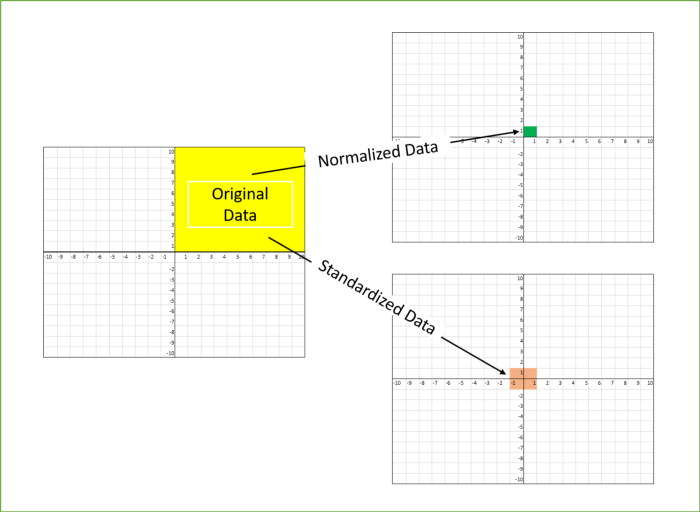
\includegraphics[width=0.8\textwidth]{img/normalisation.png}
	\end{center}
	\caption{Scaling}
\end{figure}


% ------------------------------------- %
% Développement
% ------------------------------------- %

\chapter{Développement de l’architecture}

\section{Technologies utilisées}

\subsection{Jupyter notebook}

Les notebooks Jupyter offrent un excellent moyen d'écrire et d'itérer sur du code Python. C'est un outil incroyablement puissant pour développer et présenter de manière interactive des projets de science de données. Jupyter notebook intègre le code et sa sortie dans un document unique qui combine des visualisations, du texte, des équations mathématiques et d'autres médias riches. Le flux de travail intuitif favorise un développement itératif et rapide, faisant de Jupyter notebook un choix de plus en plus populaire au cœur de la communauté de la science des données contemporaine et de l'analyse des données.

\subsection{Tensorflow}

Ce serait un défi de nos jours de trouver un ingénieur en apprentissage automatique qui n'a rien entendu sur TensorFlow. Initialement créé par l'équipe Google Brain à des fins internes, telles que le filtrage du spam sur Gmail, il est devenu open-source en 2015.

Tensorflow est souvent utilisé pour résoudre des problèmes d'apprentissage profond et pour la formation et l'évaluation des processus jusqu'au déploiement du modèle. Outre les objectifs d'apprentissage automatique, TensorFlow peut également être utilisé pour créer des simulations, basées sur des équations dérivées partielles. C'est pourquoi il est considéré comme un outil polyvalent pour les ingénieurs en apprentissage automatique.

\subsection{Keras}

Keras est une API de réseau neuronal open source écrite en Python. Il peut fonctionner sur plusieurs frameworks d'apprentissage en profondeur et d'apprentissage automatique, notamment TensorFlow, Microsoft Cognitive Tool (CNTK) et Theano.
Keras est une interface plutôt qu'un framework autonome comme TensorFlow. Il offre des abstractions intuitives de haut niveau qui permettent une expérimentation rapide.

Keras est utilisé par environ 200 000 utilisateurs, allant des chercheurs universitaires et des ingénieurs des startups et des grandes entreprises aux étudiants diplômés et aux amateurs. Keras est utilisé chez Google, Netflix, Uber, Microsoft, Square et de nombreuses startups travaillant sur la grande variété de problèmes d'apprentissage automatique.

\section{Modèles d'apprentissage}

Avant toute chose, il nous faut commencer par définir un réseau de neurones. Nous avons eu le choix entre plusieurs types de réseau. Ils diffèrent par plusieurs paramètres :

\begin{itemize}
\item la topologie des connexions entre les neurones ;
\item la fonction d’agrégation utilisée (somme pondérée, distance pseudo-euclidienne...) ;
\item et bien d'autres paramètres qui nous ne serons pas très utiles dans le déroulé de ce projet.
\end{itemize}

Nous avons choisi de commencer par utiliser un réseau à maillage \textit{dense} et avec des paramètres de base. Ceci afin de simplifier, dans un premier temps, les expérimentations. Un réseau à maillage \textit{dense} est un réseau tel que chaque neurone d'une couche est relié à tous les neurones de la couche précédente et de la couche suivante.

\begin{figure}[!h]
	\center
	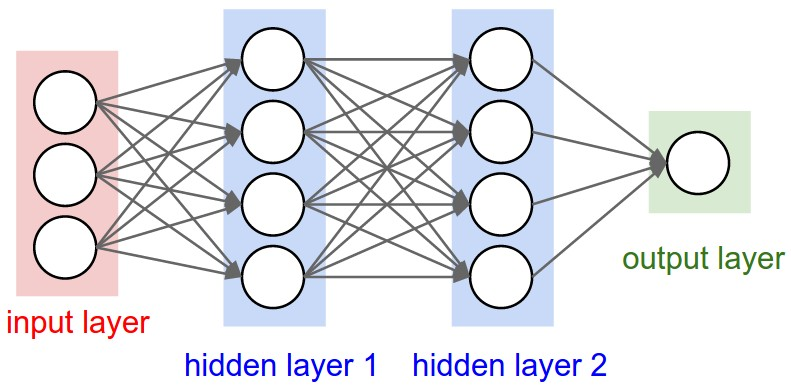
\includegraphics[width=0.7\textwidth]{img/ann-dense.jpg}
	\caption{Réseau de neurones à maillage \textit{dense}}
	\label{dense}
\end{figure}


Puis dans un deuxième temps, nous pourrons changer de modèle afin de passer à un réseau de neurones à convolution\footnote{Le CNN est un type de réseau de neurones artificiels acycliques, dans lequel le motif de connexion entre les neurones est inspiré par le cortex visuel des animaux.}(ou CNN). Ils consistent en un empilage multicouche de perceptrons, dont le but est de prétraiter de petites quantités d'informations. Les réseaux neuronaux convolutifs ont de larges applications dans la reconnaissance d'image et vidéo.

\begin{figure}[!h]
	\center
	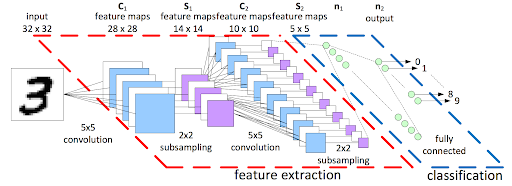
\includegraphics[width=0.8\textwidth]{img/cnn.png}
	\caption{Réseau de neurones à convolution}
\end{figure}

Afin d'abstraire l'utilisation des réseaux de neurones dans notre Notebook Jupyter, nous avons défini une classe Python (nomée \textit{MTQModel}) paramétrable qui se charge de construire un modèle, de l'entraîner et d'extraire les signatures. Point qu'on va aborder plus en détails dans la section qui suit.

\section{Signature}

Nous avons défini un réseau de neurones à maillage \textit{dense} avec deux couches cachées, comme à la figure \ref{dense}. La première couche cachée est composée de 32 neurones, la deuxième de 64. Une image qui traverse ce réseau laisse une signature $S$ qu'on peut définir comme un vecteur $H_1$ de 32 valeurs, associées à la première couche et un vecteur $H_2$ de 64 valeurs, associées à la deuxième couche. La signature d'une image dans un réseau est donc définie ainsi : $ S = (H_1, H_2)$

Afin d'extraire la signature de chaque image, nous avons intégrer une méthode à notre classe Python \textit{MTQModel}\footnote{La méthode en question s'appelle \textit{get\_hidden\_layers\_outputs(x)}} qui permet de le faire automatiquement pour chaque image du \textit{dataset}.

\subsection{Clustering}

Une fois la signature des images extraite, nous passons à l'analyse de ces dernières. Pour cela, nous utilisant un algorithme de \textit{clustering}\footnote{ou le \href{https://fr.wikipedia.org/wiki/Partitionnement_de_donn\%C3\%A9es}{Partitionnement de données} en français}, le \textbf{K-means}. Ce dernier prend en paramètres les données et un certain $K$ donnée par l'utilisateur, puis construit $K$ clusters qui regroupent les données qui sont proches\footnote{Proche en terme de distance euclidienne}.

\begin{figure}[!h]
\center
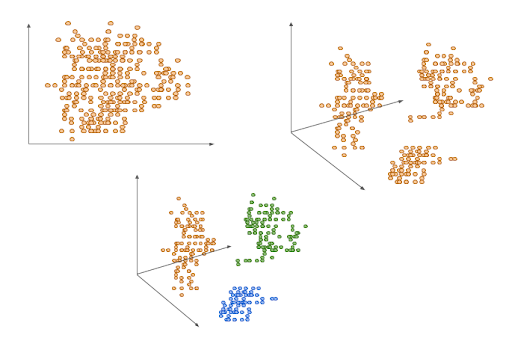
\includegraphics[width=0.8\textwidth]{img/kmeans.png}
\caption{Clustering en action}
\end{figure}

Afin de choisir un $K$ optimal, nous avons utilisé la méthode \textit{Silhouette} qui consiste à calculer, pour chaque $K$ de 2 à 10, la moyenne du score \textit{Silhouette} du clustering. Le meilleur $K$ étant celui qui donne la meilleure moyenne. Le score \textit{Silhouette} $ s(i) $ mesure combien un point est proche de son cluster comparer aux autres clusters\footnote{C'est pour cela que $ K $ doit être supérieur ou égal à 2}. Concrètement, le score d'un point $i$ est $ s(i) = \frac{b(i) - a(i)}{max(a(i), b(i))} $ avec $a(i)$ est la mesure de la similarité du point $i$ avec son cluster et $b(i)$ le mesure de dissemblance du point $i$ par rapport aux autres clusters.

\section{Interface de visualisation}
Pour pouvoir voir, analyser, évaluer et faire des expérimentations sur nos modèles, il faut avoir une interface de visualisation qui permet la projection des différentes visualisations des données et de pouvoir faire le lien entre ces visualisations.
Notre but était de pouvoir projeter le résultat de nos extractions de signatures avec UMAP et le diagramme de Sankey et de pouvoir sélectionner un ou plusieurs éléments à partir de UMAP pour suivre sa ligne dans le diagramme de Sankey et vice-versa.
Pour enfin réaliser une application web qui nous permet de faire plusieurs expérimentations, on va commencer par découvrir ce qui est UMAP et le diagramme de Sankey.
\subsection{UMAP (Uniform Manifold Approximation and Projection)}
La réduction de dimensionnalité est un outil puissant permettant aux praticiens de l'apprentissage automatique de visualiser et de comprendre des ensembles de données volumineux et de grande dimension. L'une des techniques de visualisation les plus largement utilisées est UMAP.
UMAP, à sa base utilise des algorithmes de mise en page graphique pour organiser les données dans un espace de faible dimension. Dans le sens le plus simple, UMAP construit une représentation graphique de haute dimension des données puis l'optimise en un graphique de faible dimension pour être aussi structurellement similaire que possible. Dans notre cas, on va passer de 32 et 64 dimensions à 2 dimensions.
\begin{figure}[!h]
\center
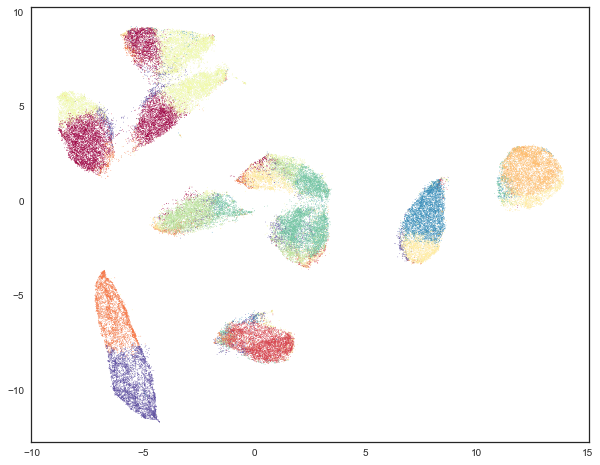
\includegraphics[width=0.8\textwidth]{img/UMAP.png}
\caption{UMAP visualisation}
\end{figure}

\subsection{Diagramme de Sankey}
Un diagramme de Sankey est un type de diagramme de flux dans lequel la largeur des flèches est proportionnelle au flux représenté.
Les diagrammes de Sankey visualisent les contributions à un flux en définissant la source pour représenter le nœud source, la cible pour le nœud cible, la valeur pour définir le volume du flux et le label indiquant le nom du nœud. Dans notre cas, on a utilisé le diagramme de Sankey pour visualiser le chemin de chaque donnée (image), en démarrant de l'input layer, en passant de son cluster de chaque couche cachée du modèle et en arrivant à l'output layer (la prédiction).

\begin{figure}[!h]
\center
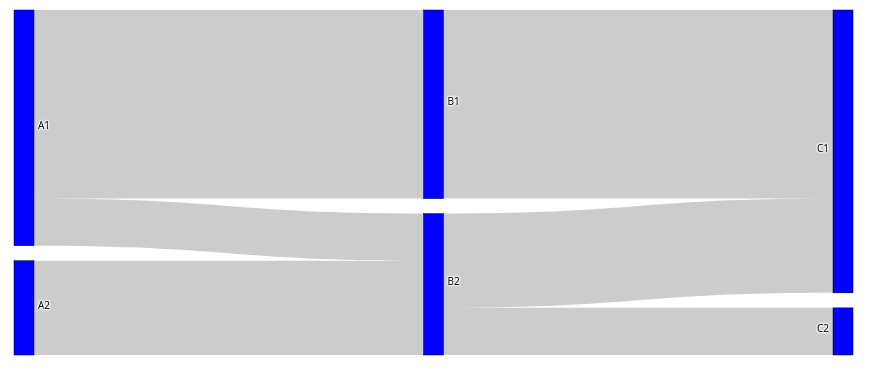
\includegraphics[width=0.8\textwidth]{img/sankey.png}
\caption{Exemple diagramme de Sankey}
\end{figure}

\subsection{Application web}
Pour concevoir une application web, on a utilisé l'outil \textit{Voilà}, qui permet de transformer un notebook jupyter en une application web autonome. Nous sommes parties d'un notebook présentant les différentes visualisations afin de générer une page web.




Voilà permet aussi de changer l'interface graphique de la page d'accueil grâce à des templates, on a donc créer notre propre template pour avoir une page d'accueil personnalisée à notre goût, qui présente nos différentes expérimentations.

% ------------------------------------- %
% Analyse des résultats
% ------------------------------------- %

\chapter{Analyse des résultats}

% ------------------------------------- %
% Annexes
% ------------------------------------- %

\appendix
\chapter{Annexe}

\section{...}

\section{...}

\chapter{Bibliographie}


\end{document}
